\section{The Necron Tombworlds}


\subsection{Building a Necron Army}

In games of the Horus Heresy: Age of Darkness, the models under a given player’s control are referred to as that player’s army. Each army is composed of a single Force Organisation chart (most commonly using the Crusade Force Organisation chart), which will include one or more Detachments. An army whose Primary Detachment is selected from any Army List is considered to have the Faction of that Primary Detachment (for example, an army whose Primary Detachment was selected from the Necrons List would be considered an Necron army). Units from various Sub-factions cannot be mixed in the same Detachment, unless a Special Rule or other ability permits this.

Other, non-Primary, Detachments in the same army may be selected from any other Army List - following any additional restrictions applied, such as the ones on the next page - but each Detachment may only include units from a single Army List, unless another Special Rule states otherwise.

When selecting a Primary Detachment, you must also choose a Sub-Faction for that detachment, in the form of a Necron Dynasty. Each Dynasty provides special bonuses and options for their units and determines the Alliance Levels between other Sub-Factions.

In addition, each Dynasty has a number of allied units that are usually attached to its Tomb Worlds, whether that be Triarch Praetorians watching over the slumbering necrons, a Destroyer Cult filling part of their ranks, or Flayed Ones lurking at the fringes. As such, a Primary Detachment is also allowed to incorporate a number of Allied Units without requiring an entire Allied Detachment be taken, so long as the number of points spent on Triarch, Destroyer, and Flayed models does not exceed 25\% of the army's total points.

\newpage
\subsection{Force Organisation Charts and Detachments}

The maximum and minimum number of units that may be included in a given army is defined by a Force Organisation chart, of which there is one basic chart available, the Crusade Force Organisation chart. 

Any Force Organisation chart is made up of one or more Detachments. A Force Organisation chart will always include one Primary Detachment, which must be selected, and may also include a number of optional Detachments which a player may choose to use or ignore. Each Detachment that a player chooses to use as part of their army must use a single Army List, which determines the Faction of that Detachment. Most optional Detachments are not required to be the same Faction as the Primary Detachment, but some Detachments may have special rules which require them to be of a certain Faction (and thus use a specific Army List). Detachments of different Factions in the same army will have additional special rules that determine how they interact (see \hyperref[allies]{the Allied Section}).

Each Detachment is composed of a number of boxes, each linked to one of the Battlefield Roles. Each of these boxes allows the player to make one selection from the section of their Army List that includes units of the same Battlefield Role. Dark boxes indicate Compulsory selections, which must be included as part of the Detachment, while the lighter boxes indicate optional choices, which are only included as part of the Detachment if the player in question chooses to do so.

Sometimes, a single choice in a Detachment may allow you to select more than one unit, or to vary the Battlefield Role of the unit selected. In all cases, such deviations from the normal procedure will be fully explained in the Force Organisation chart that the Detachment is part of.
 
Each unit selected to fill a box in any single Detachment must be chosen from the same Army List, and must be of the same Battlefield Role as that of the box. The unit profile in the Army List will dictate the number of points from the points limit that must be spent to add the unit to the player’s army. Players continue to spend points to fill boxes in Detachments within the chosen Force Organisation chart until either they run out of points, fill all boxes in all available Detachments or the player chooses to stop.

\subsection{Nodal Command Force}

The legions of a Tomb World appear to have no permanent organizational structure. Each battle, campaign and Harvest causes a specific response from the Tomb World's controlling program leading to an ever-changing chain of command. This is made possible by the Nodal Command system. A Nodal Command system allocates a hierarchy to all of the elements within it, and subsequently gives a greater operational, and decision- making, capacity to certain nodes before slaving lower ranking portions of the system to these nodes.

In battle, Necron Lords form the nodes of this structure and are assigned a hierarchical value which may change over time. As this hierarchy allows for simultaneous control of a large number of Necrons by a high ranking node, while still allowing independent reaction at the level of a Necron Warrior, it allows precise organization of the Necron force as a whole while also allowing detached groups to analyze, and react to, unforeseen situations independently.

When selecting the Nodal Command Force as your Primary Detachment, you must also determine the level at which the Tomb World is operating at. This level determines what Force Organisation slots are available to you alongside what units are considered compulsory. When selecting a higher level, you must take all of the compulsory options for that level and all levels below it. For example, selecting a Decurion Formation has a Compulsory list of: 1 HQ (Silver), 1 HQ (Bronze), 2 Troops. Compulsory units for levels above yours are \textit{not} Compulsory, you may not include any Force Organization slots above your level at all — the Tomb World has not woken up to that degree.

\subsubsection{Necron Line Formation (Bronze Command)}

The main bulk of a Necron fighting force, a Bronze level command makes up various formations led by Bronze level Lords. By themselves, these formations are usually the first coalescent response to a Tomb World's invaders, summoned when a Primary Awakener Force encounters threats too potent or complex for them to handle. 

The actual formation does vary by Tomb World and Dynasty, however each Line Formation generally contains its Bronze level Lord, a number of Phalanxes of Dynastic Warriors — or occasionally Immortals — that are supported by a small number of specialized assets such as Cyptek Conclaves, Destroyer Cults, Flayed Ones, Canopteks, and Triarch overseers, all allocated by the Tomb World and the Lord themselves.

When part of a Decurion, the usual formation is to appoint four Bronze level Lords to each Decurion, including one or more Line Formations led by the lords.

The Compulsory Headquarters unit for Necron Line Formations \textit{must} have the \quickref{Nodal Command} (Bronze) special rule.

\textbf{Primary Detachment: Necron Line Formation (Required)}
\begin{itemize}
	\item \textbf{Compulsory:} 1 HQ (Bronze),  1 Troop
	\item \textbf{Optional:} +2 Troops, +1 Elite, +2 Fast Attack, +1 Heavy Support, +4 Fortification
\end{itemize}

\subsubsection{Necron Decurion Formation (Silver Reserve Command)}

If threats are particularly potent or worthy, a high ranking or competent Lord will be appointed as Nemesor for a campaign, taking place as the overseeing Silver level Nemesor Lord for a Decurion. These oversee a number of Legions made up of Line Formations, each of which are managed by Bronze level Lords as described above. The actual Decurion is a much larger and more competent fighting force than the Line Formation Legions, with further access to superior units and specialized resources as the Tomb World is able to make them available.

As part of a greater Tesserarion, there may be one or more Decurions, however their leadership varies wildly between organizations. Some prefer to maintain a single competent Lord in control of all Decurions, while other formations call for one Silver level Lord for each Decurion.

The Compulsory Headquarters unit for Necron Decurion Formations \textit{must} have the \quickref{Nodal Command} (Silver) special rule.

\textbf{Primary Detachment: Necron Line Formation (Required)}
\begin{itemize}
	\item \textbf{Compulsory:} 1 HQ (Silver),  1 Troop
	\item \textbf{Optional:} +1 HQ, +2 Troops, +2 Elites, +1 Fast Attack, +1 Heavy Support
\end{itemize}

\subsubsection{Necron Tesserarion Formation (Gold Priority Command)}

The highest level command structure for a Necron force, it is usually led by a Tomb World's Overlord themselves after taking upon the title of Nemesor for the campaign. In particularly rare cases, this may be led by a Platinum level element in the form of a Phaeron — extremely influential and powerful Overlords that lead many worlds, even entire Dynasties — alongside his court of three Gold level Overlords chosen to direct the campaign. The Priority Command directs the Tesserarion element, fielding its largest and most powerful war machines and forces to war.

The Compulsory Headquarters unit for Necron Tesserarion Formations \textit{must} have the \quickref{Nodal Command} (Gold) special rule.

\textbf{Primary Detachment: Necron Line Formation (Required)}
\begin{itemize}
	\item \textbf{Compulsory:} 1 HQ (Gold)
	\item \textbf{Optional:} +1 HQ, +1 Phaeron, +1 Troops, +1 Elite, +1 Fast Attack, +2 Heavy Supports
\end{itemize}
 
\newpage
{
\centering
\textbf{Nodal Command Force Detachment}

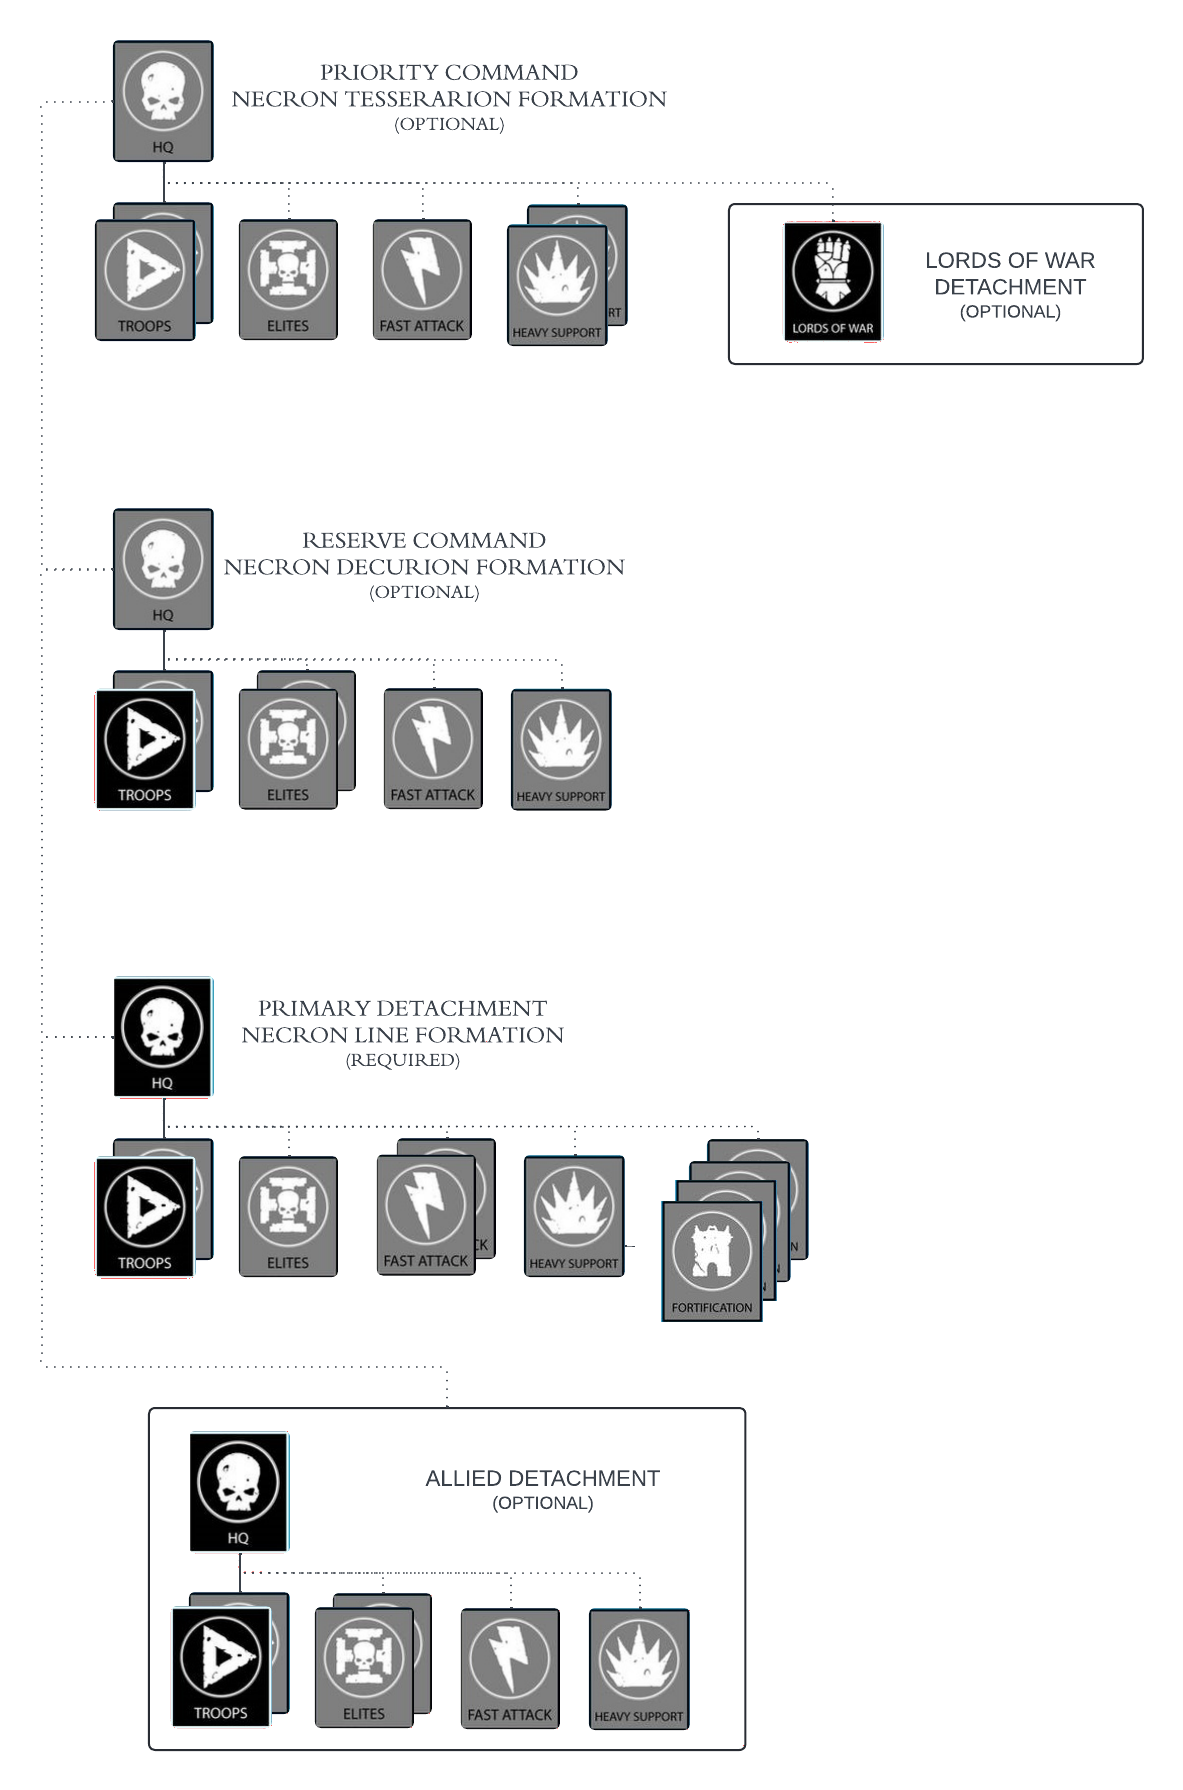
\includegraphics[width=470pt, height=700pt]{Org chart.png}

\begin{figure}
	\centering
	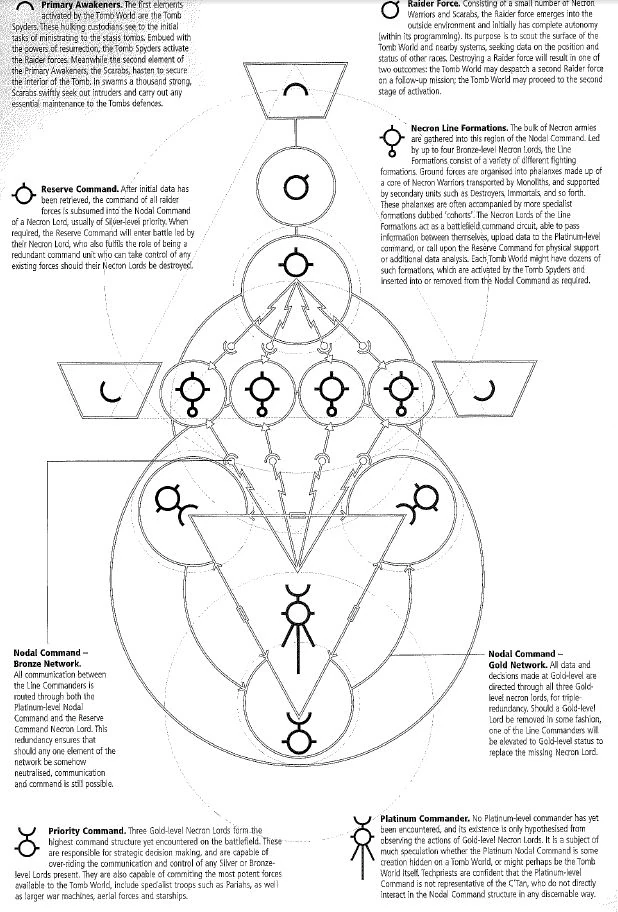
\includegraphics[width=515pt, height=750pt]{nodal.png}
\end{figure}
}